% 由 gen_paper.py 从 results.json 自动生成，请勿手改数字
% 编译：xelatex demo.tex （跑两趟）
\documentclass[12pt]{article}
\makeatletter
\def\input@path{{../../templates/}}
\makeatother
\usepackage{cumcm-paper}

\begin{document}
\cumcmtitle{区域农产品仓储选址与配送网络优化}

\begin{abstract}
随着区域农产品产量的持续增长，原有仓储与配送体系已接近饱和，如何在预测未来产量的基础上科学选址并优化配送网络，是降低流通损耗、提升供应链效率的关键问题。本文针对产量预测、仓址评选与配送网络优化三个子问题，建立了灰色预测、熵权--TOPSIS 综合评价与图论--线性规划相结合的模型体系。

针对问题一，我们建立了 GM(1,1) 灰色预测模型。原始序列 2021 年数据缺测，先用线性插值补全，经四分位距法检验区间 $[86.50, 216.50]$ 内无异常值。考虑到样本仅 6 个数据点、不适用 ARIMA，选用适合小样本指数趋势的 GM(1,1)。级比检验显示全部级比落在可容覆盖区间 $[0.7515, 1.3307]$ 内，模型适用。求解得发展系数 $a=-0.0833$、灰作用量 $b=117.4371$，拟合优度 $R^2=0.9992$，均方根误差 0.6398 万吨，平均绝对百分比误差 0.3592\%，精度等级为一级。预测 2025 年与 2026 年产量分别为 201.6 万吨与 219.13 万吨。

针对问题二，我们建立了熵权--TOPSIS 综合评价模型，从年吞吐能力、建设投资、覆盖率与路网密度四个维度评选仓址。其中建设投资为成本型指标，需先正向化。我们比较了 $\max(x)-x$ 与倒数法 $1/x$ 两种方案：前者将该列平移至以 0 为下界，人为放大变异系数，导致投资一项的熵权高达 0.9614，综合排序几乎由单一指标决定；改用倒数法后该权重降至 0.4904，四项权重分别为 0.0525, 0.4904, 0.0146, 0.4425，评价结果更为均衡。最终三个仓址的贴近度为 甲=0.4645, 乙=0.9733, 丙=0.0267，排序为 乙 $>$ 甲 $>$ 丙，推荐选址乙。

针对问题三，我们分两层建立配送网络模型。干线铺设层以最小生成树刻画“用最小总里程连通全部节点”，Kruskal 算法求得干线总长 54 km，较全网铺设节省 99 km；应急配送层以 Dijkstra 算法求得从仓库 $W$ 到最远节点 $E$ 的最短路径为 $W \to B \to D \to E$，长度 40 km。运量分配层建立线性规划模型，以总运费最小为目标，在产能、分区需求与单点通过能力约束下求得最优方案，总运费 2280 万元。

最后对总成本模型作单因素灵敏度分析。在 $\pm 10\%$ 扰动范围内，单位运费与配送量的弹性系数均为 0.8155，固定成本为 0.1845，三者之和恰为 1，与成本函数的线性结构一致，表明模型对参数扰动的响应稳定可控。

\end{abstract}
\keywords{GM(1,1) 灰色预测；熵权法；TOPSIS；最小生成树；线性规划；灵敏度分析}

\section{问题重述}

某区域农产品流通体系面临产量增长与仓储能力不足的矛盾，需在现有基础上重新规划仓储与配送。已知 2019--2024 年该区域农产品年产量统计数据（其中 2021 年因统计口径调整数据缺测），另有三个候选仓址在年吞吐能力、建设投资、覆盖率、路网密度四项指标上的实测值，以及由仓库 $W$ 与五个配送节点 $A$--$E$ 构成的公路网络及各路段里程。现需解决：

\begin{enumerate}
  \item 补全缺测数据并预测未来两年的产量，为仓储规模决策提供依据；
  \item 在三个候选仓址中评选出综合最优者，并说明评价方法的合理性；
  \item 设计配送干线铺设方案与应急配送路径，并给出使总运费最小的运量分配方案。
\end{enumerate}

\section{问题分析}

\textbf{问题一}属于小样本时间序列预测。样本量仅 6 个，远低于 ARIMA 所需的数据量，而序列呈近似指数增长趋势，符合 GM(1,1) 的适用前提。需先处理缺测值，并在建模后进行级比检验与残差检验，否则预测结果不具备可信度。

\textbf{问题二}属于多指标综合评价。四项指标量纲不一且方向不同（建设投资越小越好，其余越大越好），需先统一方向再赋权。考虑到权重应反映数据本身的区分度而非主观判断，选用熵权法客观赋权，再以 TOPSIS 计算各方案与理想解的相对贴近度。此处正向化方式的选择会实质影响权重分布，需要专门论证。

\textbf{问题三}是复合优化问题，包含三个相互独立的子目标：干线铺设求“最小代价连通所有节点”，对应最小生成树；应急配送求“两点间最短距离”，对应最短路；运量分配求“线性目标下的资源最优配置”，对应线性规划。三者可分别建模、独立求解。

上述三个问题由同一数据层支撑，预测、评价和优化结果最终在检验环节汇合，整体研究流程见图~\ref{fig:workflow}。

\begin{figure}[!htbp]
  \centering
  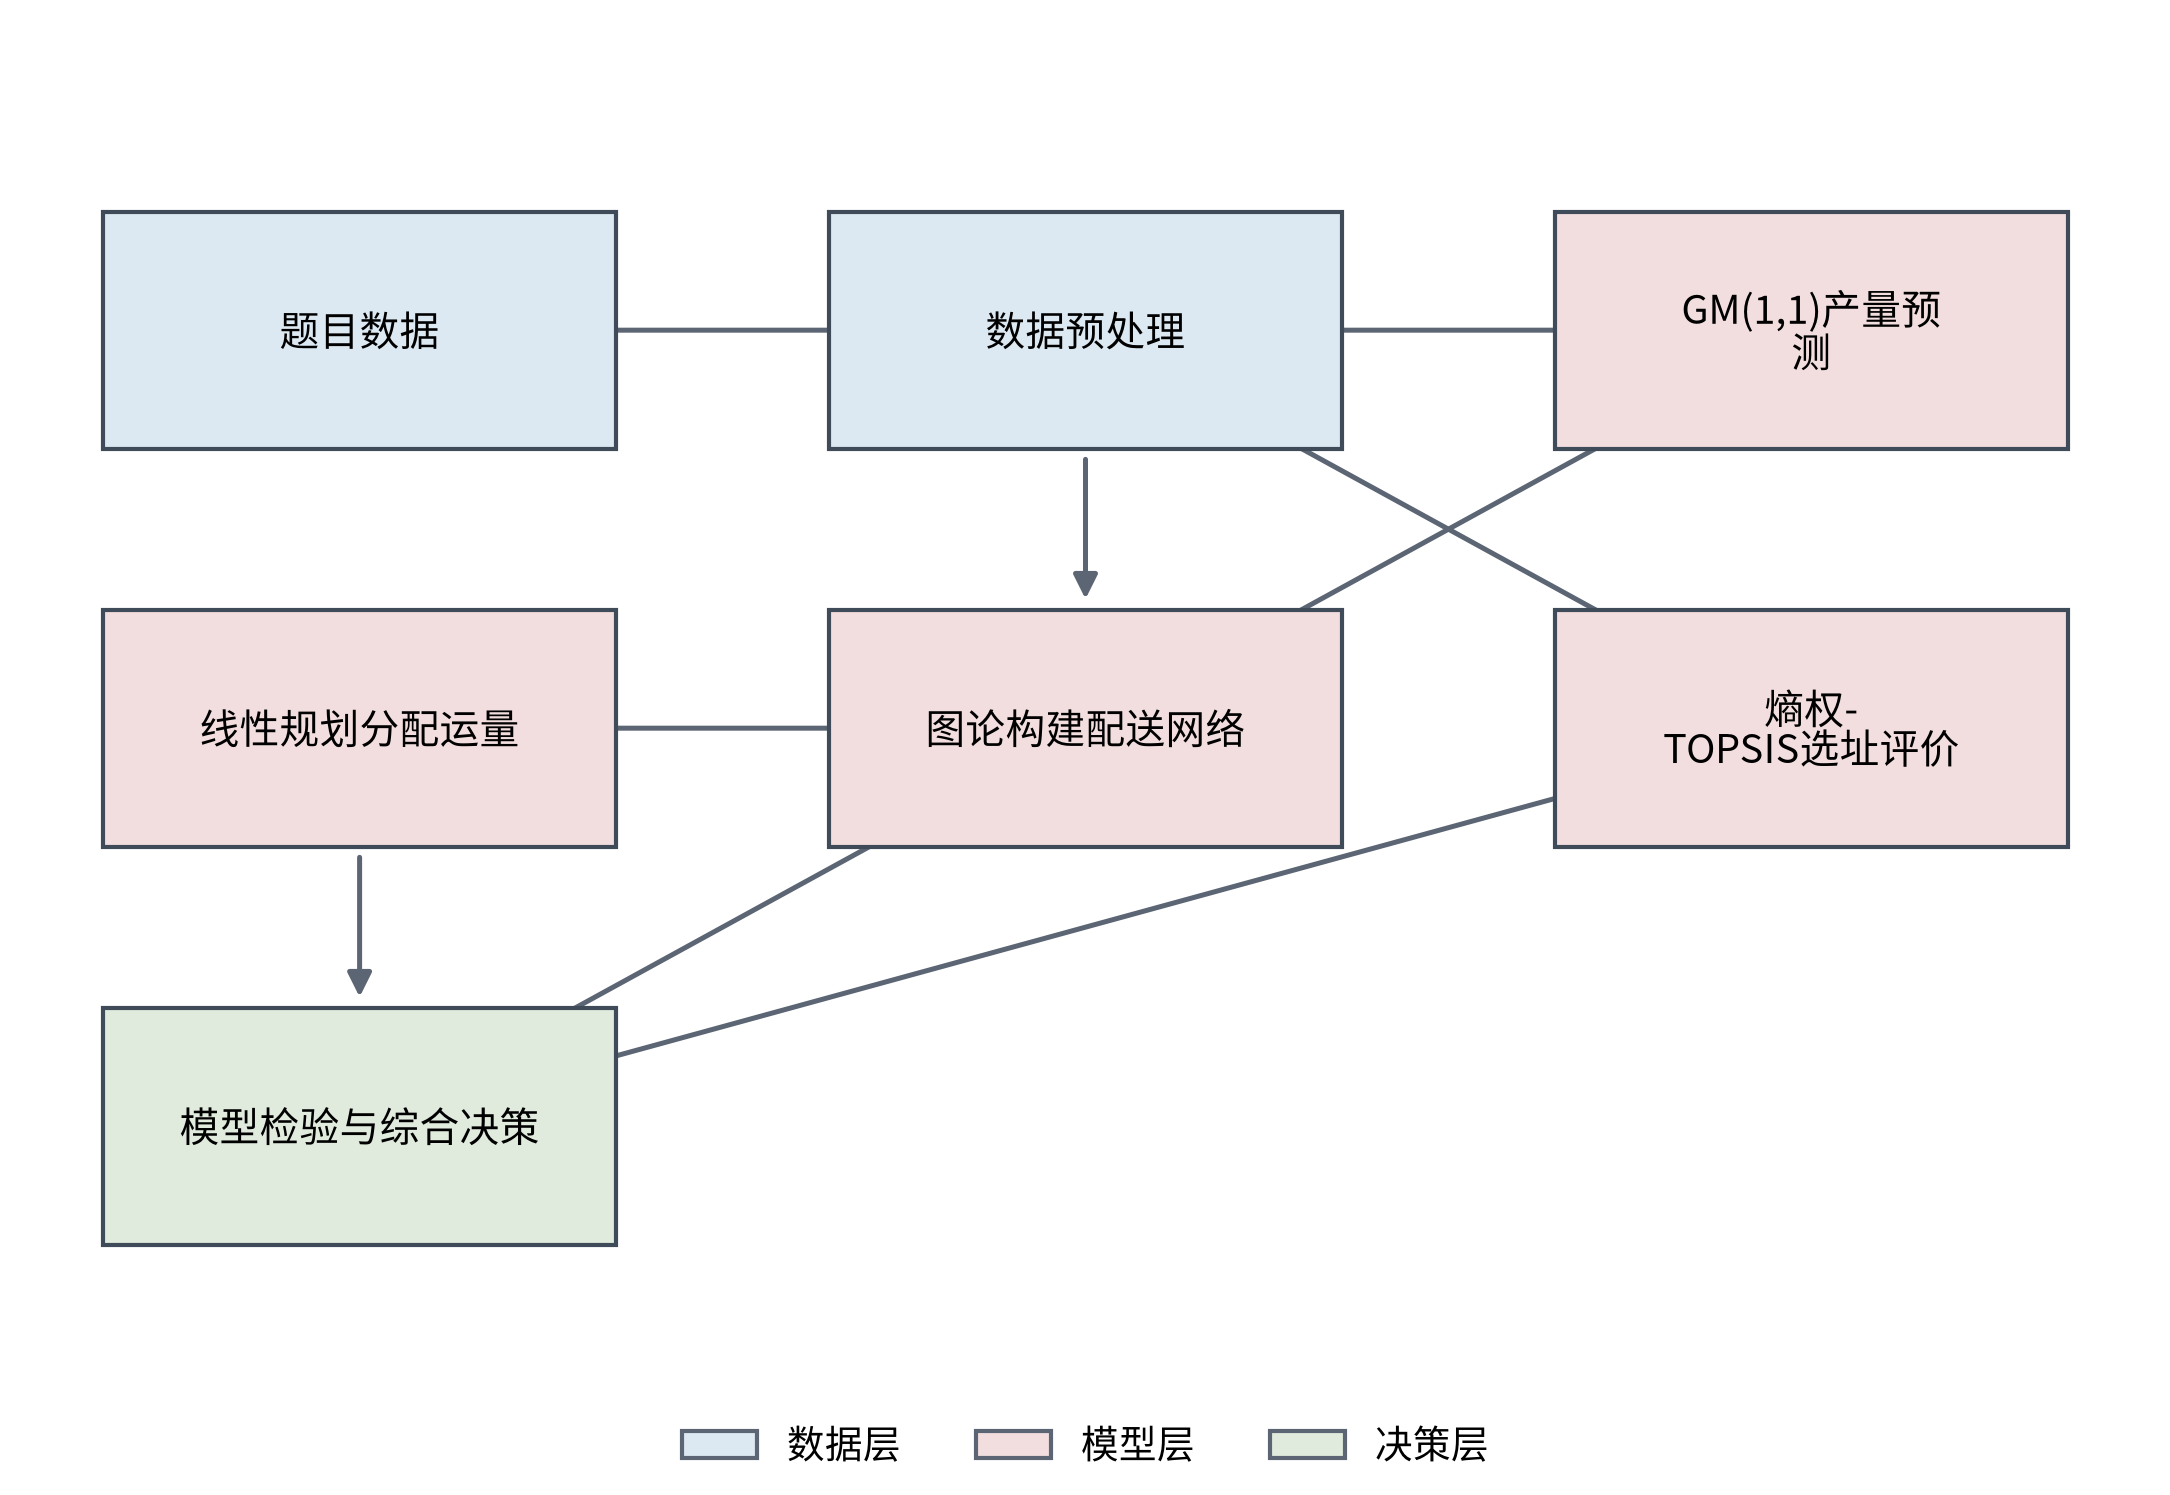
\includegraphics[width=0.88\textwidth]{fig0_workflow.png}
  \caption{区域仓储选址与配送优化的总体研究流程}
  \label{fig:workflow}
\end{figure}

\section{模型假设}

\begin{enumerate}
  \item 假设区域内农产品产量的增长主要由种植面积与单产的稳定提升驱动，不考虑重大自然灾害等突发因素；
  \item 假设 2021 年缺测数据可由相邻年份线性插值近似，即该年产量变化趋势与前后年份一致；
  \item 假设各候选仓址的四项指标在评价期内保持稳定，不随季节波动；
  \item 假设公路网络中各路段双向通行、里程对称，且运输成本与里程成正比；
  \item 假设各中转点的单位运费在其通过能力范围内保持恒定，不存在规模折扣。
\end{enumerate}

\section{符号说明}

\begin{table}[htbp]
  \centering
  \caption{符号说明}
  \label{tab:notation}
  \begin{tabular}{cl}
    \toprule
    符号 & 含义 \\
    \midrule
    $x^{(0)}(k)$ & 原始产量序列第 $k$ 期观测值 \\
    $x^{(1)}(k)$ & 一次累加生成序列 \\
    $a$ & GM(1,1) 发展系数 \\
    $b$ & GM(1,1) 灰作用量 \\
    $e_j$ & 第 $j$ 项指标的信息熵 \\
    $w_j$ & 第 $j$ 项指标的熵权 \\
    $C_i$ & 第 $i$ 个方案的相对贴近度 \\
    $T$ & 最小生成树的边集 \\
    $x_i$ & 经第 $i$ 个中转点的运量（万吨） \\
    $Z$ & 总运费目标函数（万元） \\
    \bottomrule
  \end{tabular}
\end{table}

\section{模型的建立与求解}

\subsection{问题一：基于 GM(1,1) 的产量预测模型}

\subsubsection{数据预处理}

原始序列中 2021 年数据缺测，采用线性插值补全，得该年产量 145 万吨，共填补 1 个缺失值。随后用四分位距法检验异常值，正常值区间为 $[86.50, 216.50]$，序列中无异常点（异常值个数为 0），数据可直接用于建模。

\begin{table}[!htbp]
  \centering
  \small
  \caption{2019--2024 年区域农产品产量原始数据与预处理结果（单位：万吨）}
  \label{tab:data}
  \begin{tabular}{lcccccc}
    \toprule
    年份 & 2019 & 2020 & 2021 & 2022 & 2023 & 2024 \\
    \midrule
    原始值 & 120 & 132 & 缺测 & 158 & 171 & 185 \\
    预处理后 & 120 & 132 & 145 & 158 & 171 & 185 \\
    GM(1,1) 拟合 & 120.00 & 132.90 & 144.45 & 157.01 & 170.65 & 185.48 \\
    残差 & 0.000 & -0.899 & 0.550 & 0.995 & 0.349 & -0.483 \\
    \bottomrule
  \end{tabular}
\end{table}

\subsubsection{模型建立}

设原始序列为 $x^{(0)} = \{x^{(0)}(1), \dots, x^{(0)}(n)\}$，作一次累加生成
\begin{equation}
x^{(1)}(k) = \sum_{i=1}^{k} x^{(0)}(i), \quad k = 1, 2, \dots, n .
\end{equation}
建立灰色微分方程
\begin{equation}
\frac{\mathrm{d} x^{(1)}}{\mathrm{d} t} + a x^{(1)} = b ,
\end{equation}
其中 $a$ 为发展系数、$b$ 为灰作用量。以紧邻均值生成序列 $z^{(1)}(k) = \tfrac{1}{2}\left[x^{(1)}(k) + x^{(1)}(k-1)\right]$ 构造数据矩阵，由最小二乘法估计参数，得时间响应函数
\begin{equation}
\hat{x}^{(1)}(k+1) = \left(x^{(0)}(1) - \frac{b}{a}\right) \mathrm{e}^{-ak} + \frac{b}{a} ,
\end{equation}
再作累减还原即得预测值 $\hat{x}^{(0)}(k+1) = \hat{x}^{(1)}(k+1) - \hat{x}^{(1)}(k)$。

\subsubsection{级比检验}

建模前需检验序列是否落入 GM(1,1) 的可容覆盖区间。级比定义为 $\lambda(k) = x^{(0)}(k-1) / x^{(0)}(k)$，要求
\begin{equation}
\lambda(k) \in \left(\mathrm{e}^{-2/(n+1)},\ \mathrm{e}^{2/(n+1)}\right) = (0.7515,\ 1.3307) .
\end{equation}
实际级比为 0.9091, 0.9103, 0.9177, 0.9240, 0.9243，全部落在区间内，GM(1,1) 适用。

\subsubsection{求解结果与精度检验}

求解得 $a = -0.0833$，$b = 117.4371$。由于 $|a| = 0.0833 < 0.3$，模型可用于中长期预测。拟合值与残差见表~\ref{tab:data}，精度指标为
\begin{equation}
R^2 = 0.9992, \quad \mathrm{RMSE} = 0.6398, \quad \mathrm{MAE} = 0.546, \quad \mathrm{MAPE} = 0.3592\% .
\end{equation}
MAPE 小于 1\%，属一级精度。预测 2025 年产量 201.6 万吨、2026 年产量 219.13 万吨。拟合效果与残差分布见图~\ref{fig:fit}，残差在零线两侧随机分布，无系统性偏差。

\begin{figure}[!htbp]
  \centering
  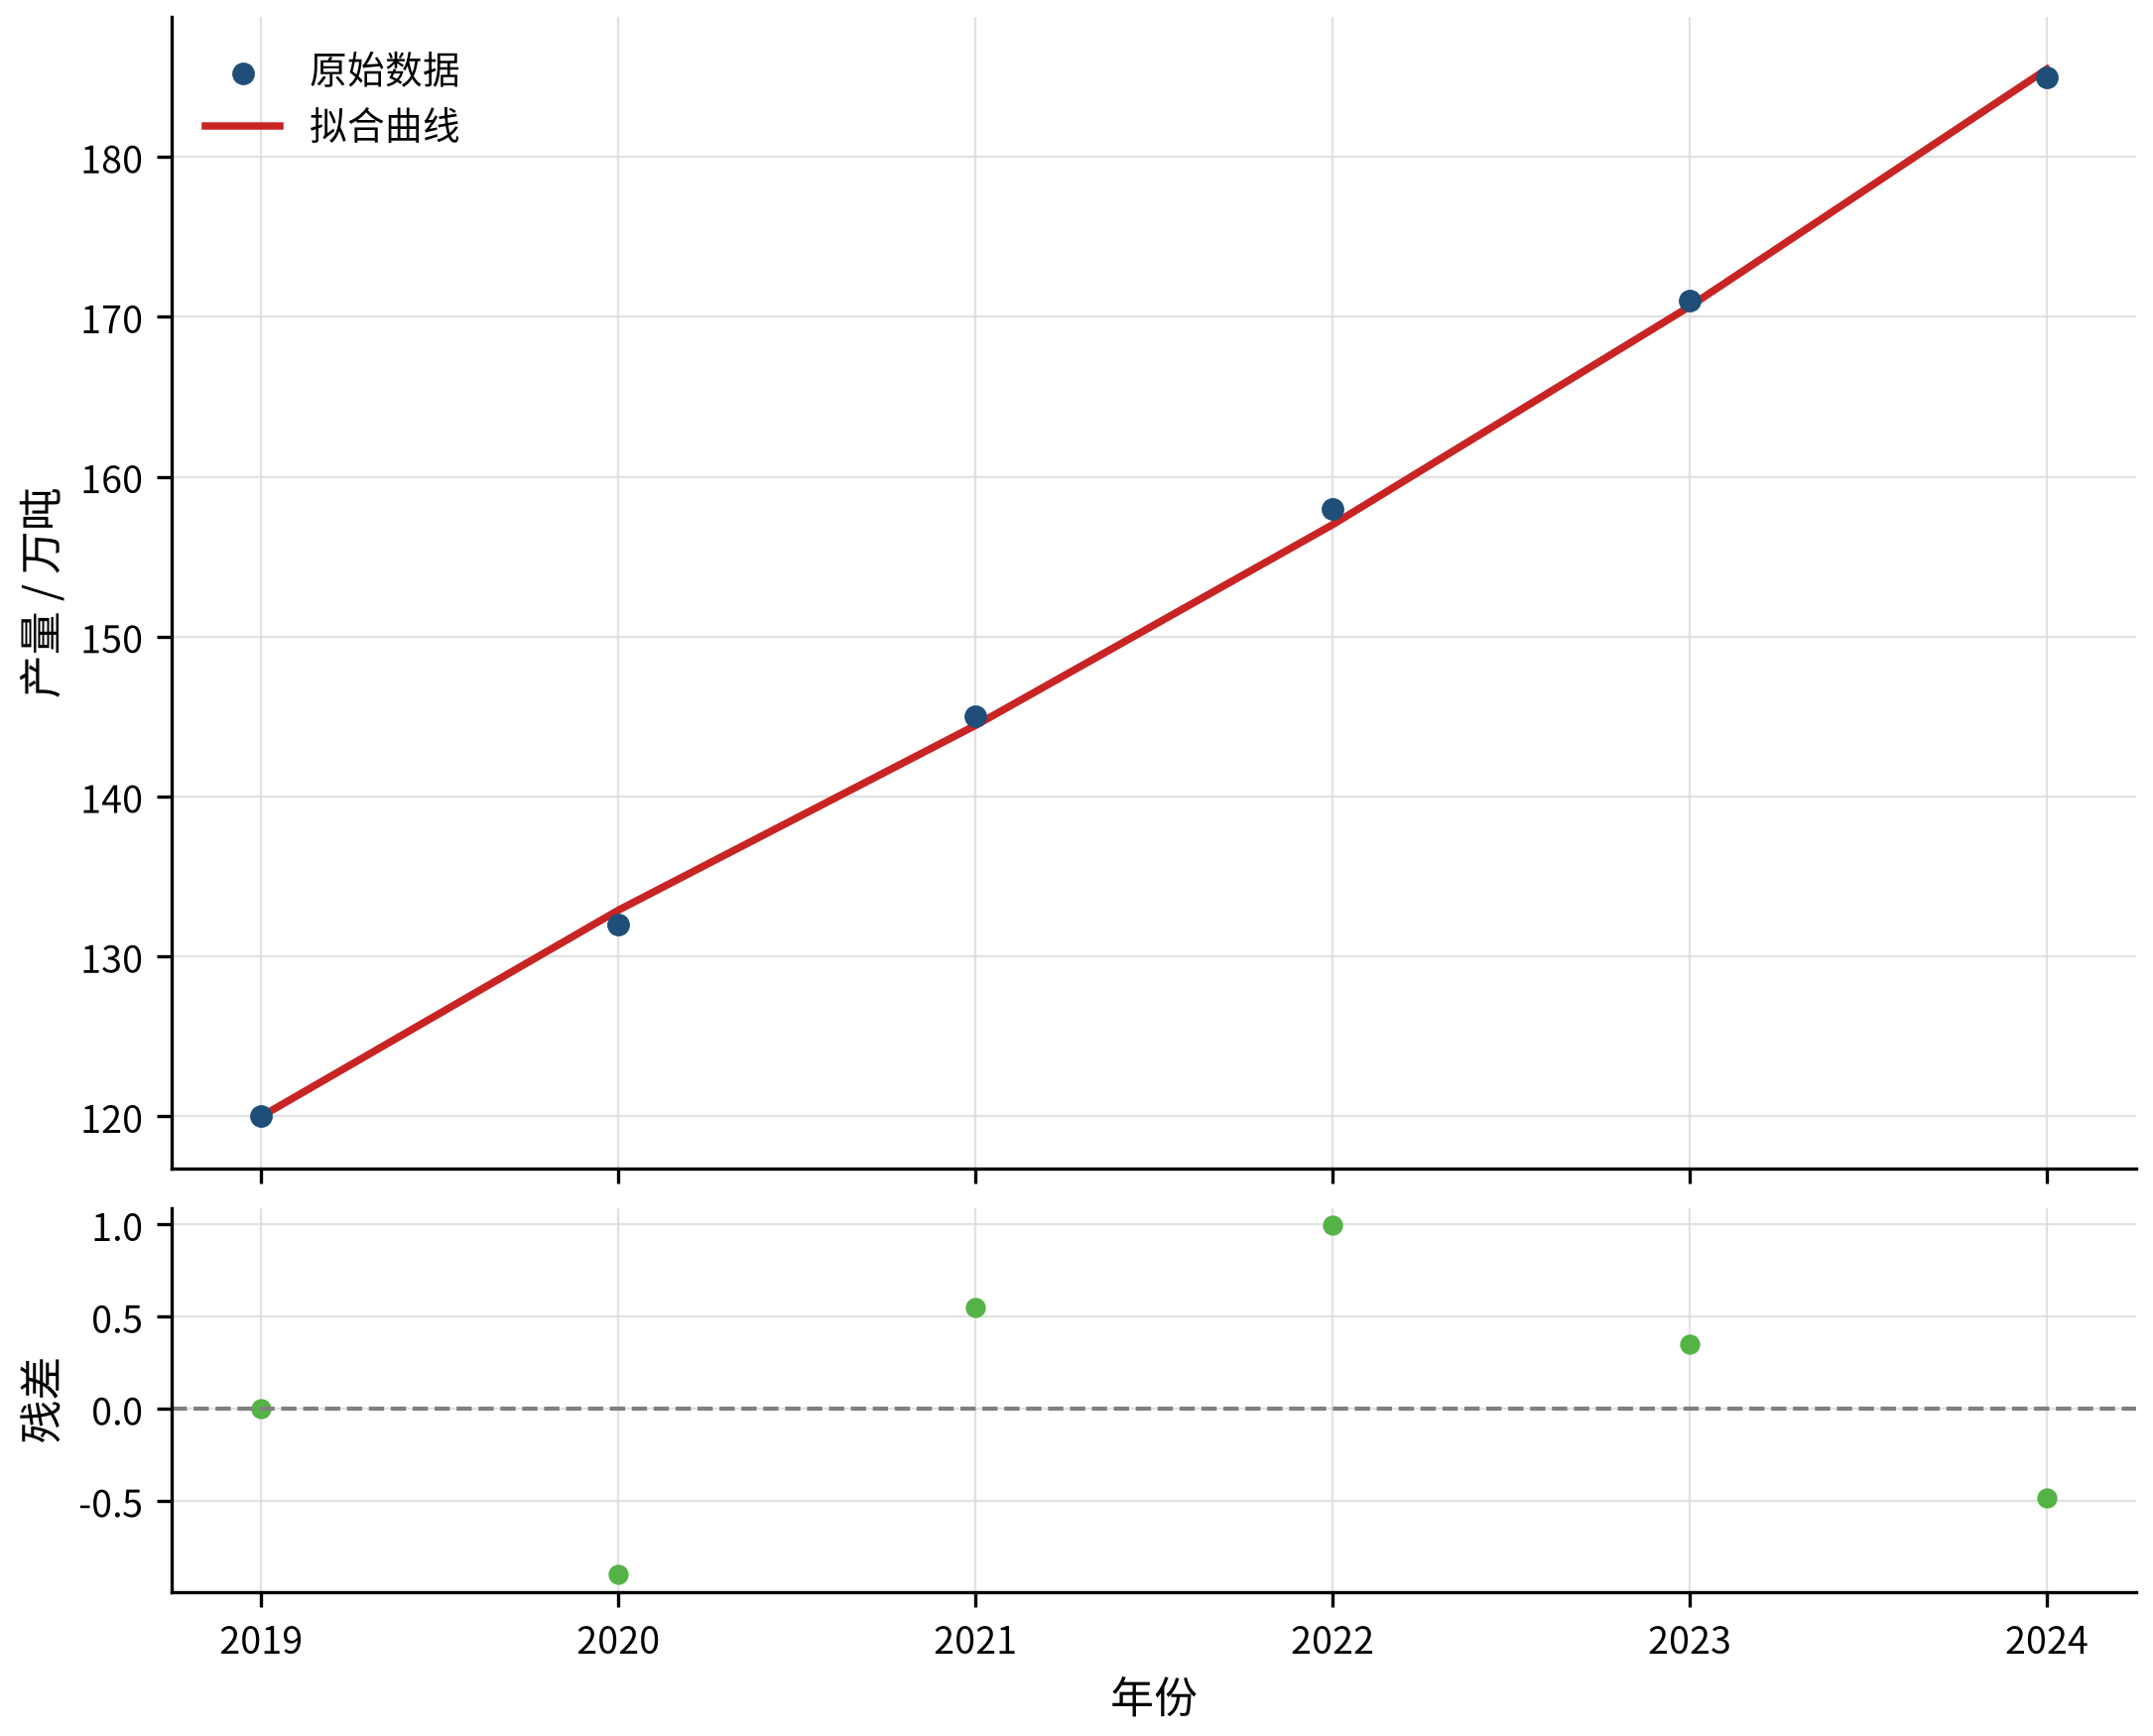
\includegraphics[width=0.75\textwidth]{fig1_fit.png}
  \caption{GM(1,1) 拟合效果与残差分布}
  \label{fig:fit}
\end{figure}

\subsection{问题二：基于熵权--TOPSIS 的仓址评选模型}

\subsubsection{原始数据与指标方向}

\begin{table}[!htbp]
  \centering
  \small
  \caption{三个候选仓址的原始指标值}
  \label{tab:matrix}
  \begin{tabular}{lrrrr}
    \toprule
    仓址 & 年吞吐能力/万吨 & 建设投资/百万元 & 覆盖率 & 路网密度 \\
    \midrule
    甲 & 185 & 42 & 0.91 & 3.2 \\
    乙 & 172 & 35 & 0.88 & 4.1 \\
    丙 & 199 & 55 & 0.95 & 2.7 \\
    \bottomrule
  \end{tabular}
\end{table}

四项指标中，建设投资为成本型（越小越好），其余三项为效益型（越大越好），需先将成本型指标正向化。

\subsubsection{正向化方式的选择}

常用的正向化方式有 $\max(x) - x$ 与倒数法 $1/x$ 两种。前者将该列平移至以 0 为下界，使其变异系数被人为放大——而熵权法正是以列内离散程度赋权，这会导致该指标权重虚高。两种方式的计算结果对比见表~\ref{tab:cmp}。

\begin{table}[!htbp]
  \centering
  \small
  \caption{两种正向化方式下的熵权与贴近度对比}
  \label{tab:cmp}
  \begin{tabular}{lrrrrrrr}
    \toprule
    & \multicolumn{4}{c}{熵权} & \multicolumn{3}{c}{贴近度} \\
    \cmidrule(lr){2-5} \cmidrule(lr){6-8}
    正向化方式 & 吞吐 & 投资 & 覆盖率 & 路网 & 甲 & 乙 & 丙 \\
    \midrule
    $\max(x)-x$ & 0.0040 & 0.9614 & 0.0011 & 0.0335 & 0.6500 & 0.9996 & 0.0004 \\
    $1/x$（本文采用） & 0.0525 & 0.4904 & 0.0146 & 0.4425 & 0.4645 & 0.9733 & 0.0267 \\
    \bottomrule
  \end{tabular}
\end{table}

可见采用 $\max(x)-x$ 时，投资一项的熵权达 0.9614，其余三项合计不足 0.0386，综合评价退化为对单一指标的排序；改用倒数法后最大权重降至 0.4904，权重分布合理。\textbf{本文采用倒数法}。需要说明的是，两种方式下最优方案均为乙，结论稳健，但贴近度的区分度差异显著。

\subsubsection{模型建立与求解}

设正向化后的决策矩阵为 $X = (x_{ij})_{m \times n}$。先作归一化 $p_{ij} = x_{ij} / \sum_{i=1}^{m} x_{ij}$，计算第 $j$ 项指标的信息熵
\begin{equation}
e_j = -\frac{1}{\ln m} \sum_{i=1}^{m} p_{ij} \ln p_{ij} ,
\end{equation}
则熵权为 $w_j = (1 - e_j) / \sum_{k} (1 - e_k)$。再作向量归一化并加权，确定正负理想解 $Z^{+}$、$Z^{-}$，计算各方案到两者的欧氏距离 $D_i^{+}$、$D_i^{-}$，得相对贴近度
\begin{equation}
C_i = \frac{D_i^{-}}{D_i^{+} + D_i^{-}} \in [0, 1] .
\end{equation}

求解得四项指标熵权为 0.0525, 0.4904, 0.0146, 0.4425，三个仓址的贴近度为 甲 $0.4645$, 乙 $0.9733$, 丙 $0.0267$，排序为 乙 $>$ 甲 $>$ 丙。\textbf{推荐选址乙}。该方案在建设投资上明显占优（35 百万元，为三者最低），路网密度亦最高（4.1），虽吞吐能力略低于丙，但综合表现最佳。

需强调的是，熵权反映的是各指标在样本内的区分度，而非指标本身的重要性，不应与 AHP 的主观权重混同解释。

\FloatBarrier

\subsection{问题三：配送网络优化模型}

\subsubsection{干线铺设：最小生成树模型}

配送干线需以最小总里程连通仓库 $W$ 与全部配送节点。设无向赋权图 $G = (V, E, w)$，求边集 $T \subseteq E$ 使
\begin{equation}
\min \sum_{e \in T} w(e) \quad \text{s.t.} \quad (V, T) \text{ 连通且无圈} .
\end{equation}
用 Kruskal 算法求解，结果见表~\ref{tab:mst} 与图~\ref{fig:net}。干线总长 54 km，相比铺设全部 10 条路段（总长 153 km）节省 99 km。

\begin{table}[!htbp]
  \centering
  \small
  \caption{最小生成树选中的干线（总长 54 km）}
  \label{tab:mst}
  \begin{tabular}{lc}
    \toprule
    干线 & 长度 / km \\
    \midrule
    $W \leftrightarrow A$ & 12 \\
    $A \leftrightarrow B$ & 9 \\
    $B \leftrightarrow C$ & 11 \\
    $B \leftrightarrow D$ & 14 \\
    $D \leftrightarrow E$ & 8 \\
    \midrule
    合计 & 54 \\
    \bottomrule
  \end{tabular}
\end{table}

\begin{figure}[!htbp]
  \centering
  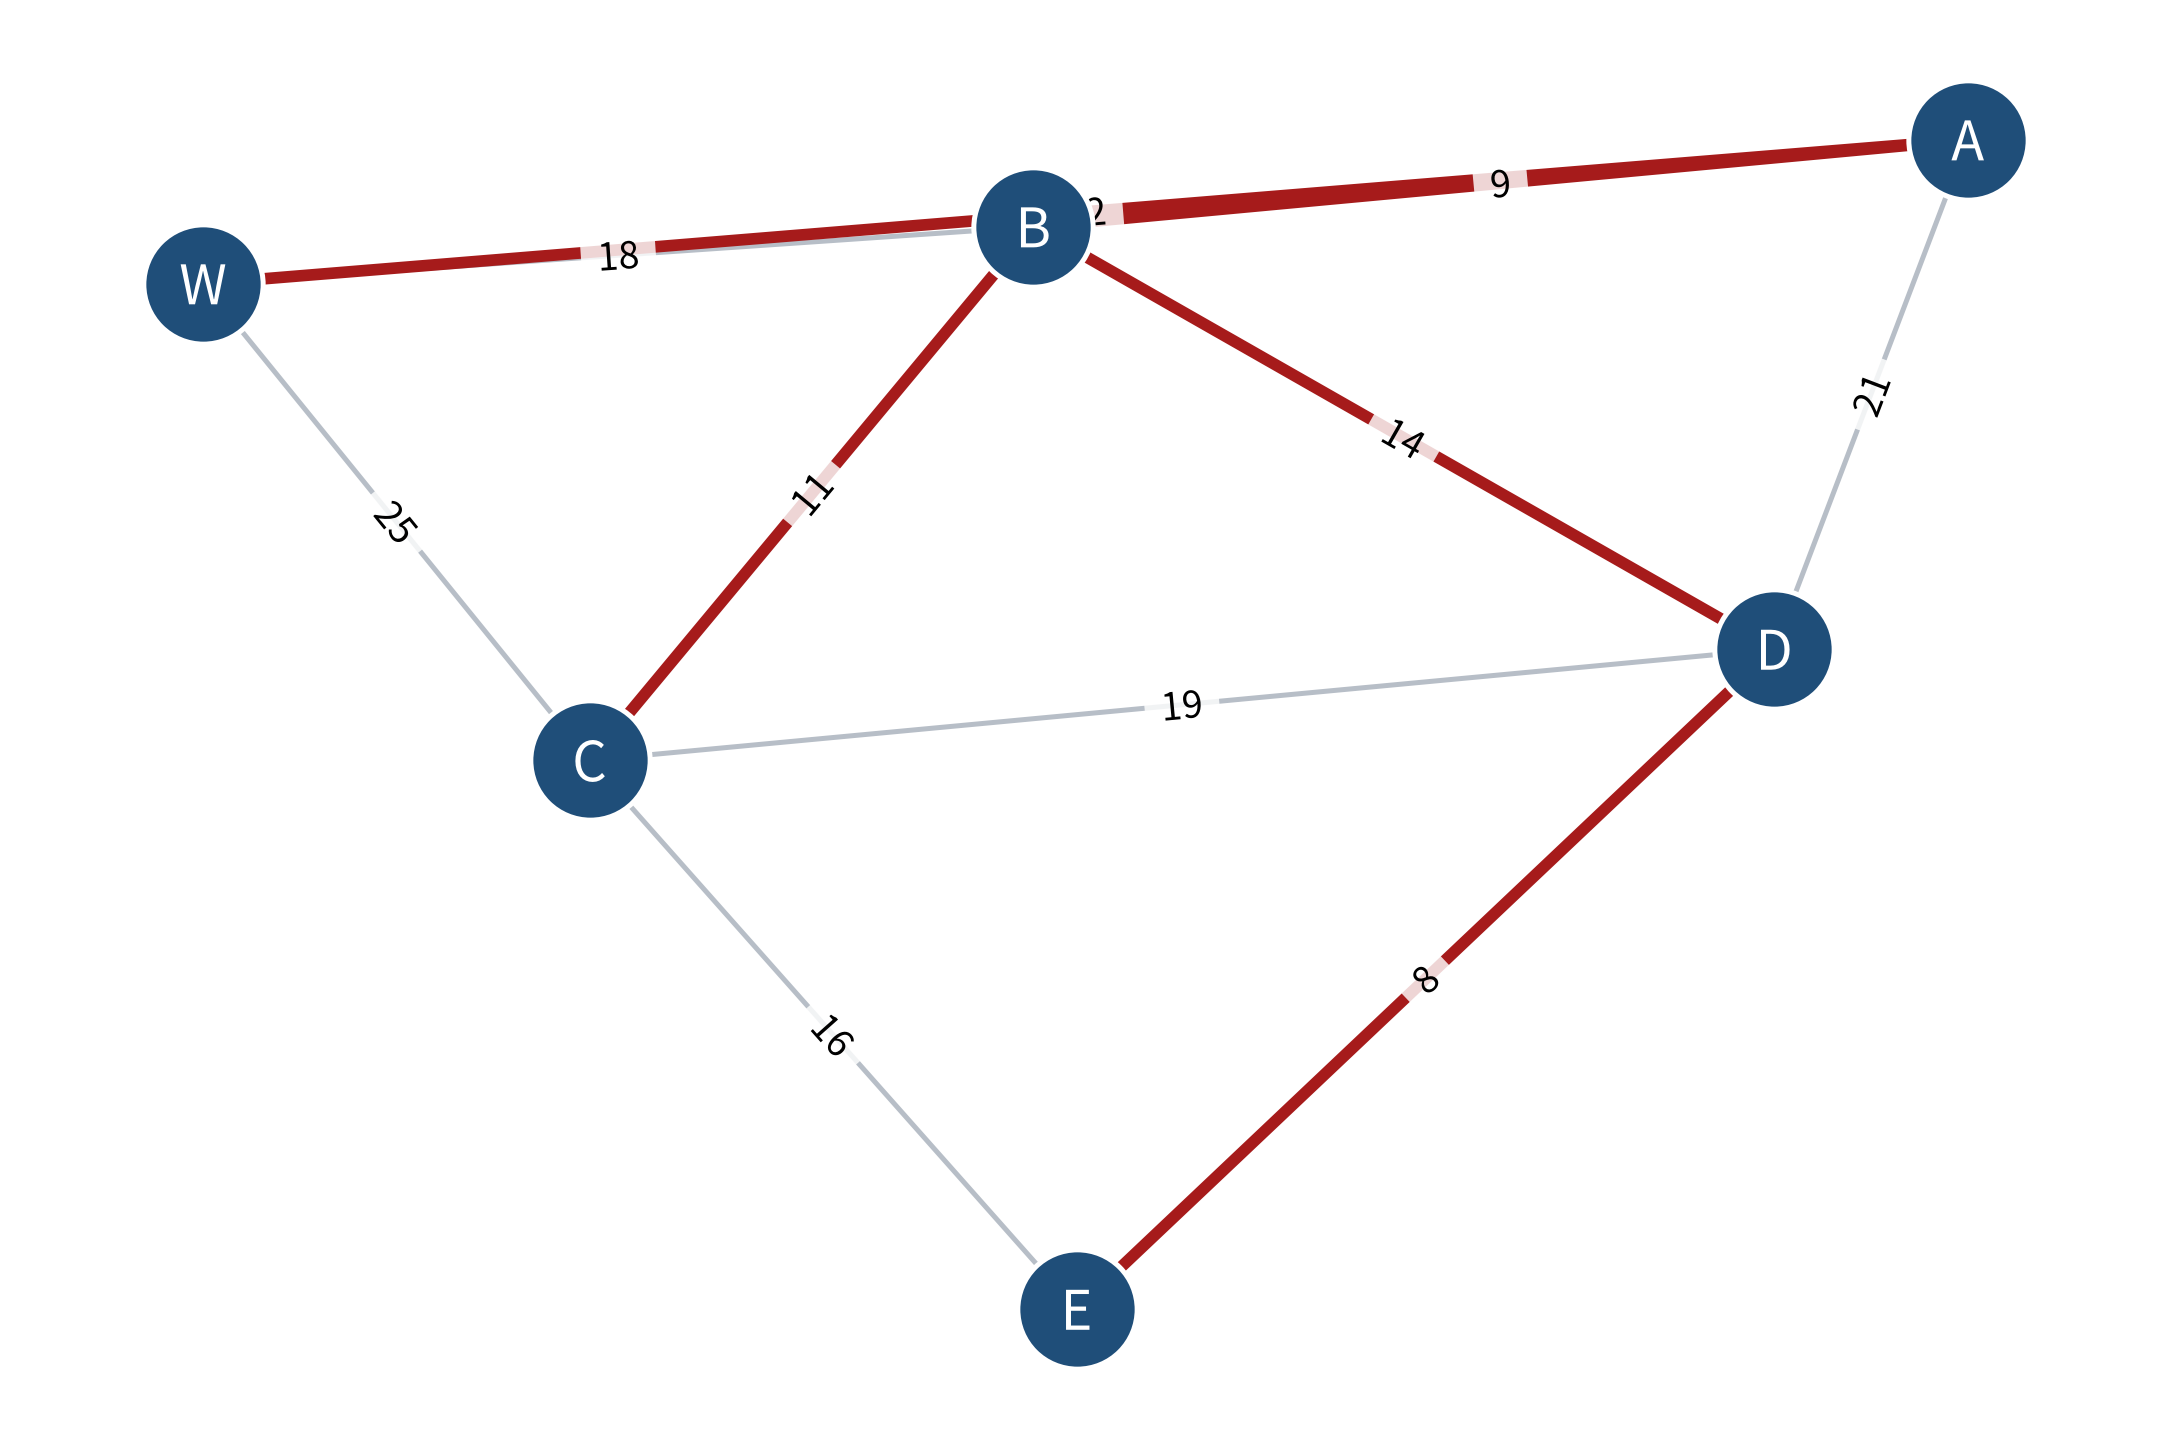
\includegraphics[width=0.8\textwidth]{fig3_net.png}
  \caption{配送网络拓扑与最小生成树干线方案}
  \label{fig:net}
\end{figure}

\subsubsection{应急配送：最短路模型}

应急情形下需快速抵达最远节点 $E$。因网络中不存在负权边，采用 Dijkstra 算法求解，得最短路径为
\begin{equation}
W \to B \to D \to E ,
\end{equation}
路径长度 40 km。注意该路径与干线方案不完全重合——干线追求全局连通成本最小，应急路径追求单点可达时间最短，两者目标不同，不应混为一谈。

\subsubsection{运量分配：线性规划模型}

设经中转点 $A$、$B$、$C$、$D$ 的运量分别为 $x_1, \dots, x_4$（万吨），单位运费依次为 12、18、25、21 万元/万吨。建立模型
\begin{equation}
\begin{aligned}
\min \ & Z = 12x_1 + 18x_2 + 25x_3 + 21x_4 \\
\text{s.t.} \ & x_1 + x_2 + x_3 + x_4 \leq 185 && \text{(总产能约束)} \\
& x_1 + x_2 \geq 80 && \text{(北片区需求)} \\
& x_3 + x_4 \geq 60 && \text{(南片区需求)} \\
& 0 \leq x_i \leq 70, \quad i = 1, \dots, 4 && \text{(单点通过能力)}
\end{aligned}
\end{equation}
用单纯形法求解，最优解为 $x = (70, 10, 0, 60)$，最小总运费 2280 万元。

\begin{table}[!htbp]
  \centering
  \small
  \caption{最优运输方案（总运费 2280 万元）}
  \label{tab:lp}
  \begin{tabular}{lrrrr}
    \toprule
    中转点 & A & B & C & D \\
    \midrule
    单位运费 & 12 & 18 & 25 & 21 \\
    分配运量 / 万吨 & 70 & 10 & 0 & 60 \\
    \bottomrule
  \end{tabular}
\end{table}

结果符合直觉：单位运费最低的 $A$ 点被优先用满至通过能力上限 70 万吨，北片区剩余需求由次低的 $B$ 承担 10 万吨；南片区则全部交由运费较低的 $D$ 点（60 万吨），运费最高的 $C$ 点不启用。

\FloatBarrier

\section{灵敏度分析}

对总成本模型 $Z = c \cdot q + F$（$c$ 为单位运费、$q$ 为配送量、$F$ 为固定成本）作单因素灵敏度分析，在基准点 $c = 12$、$q = 140$、$F = 380$ 附近按 $\pm 5\%$、$\pm 10\%$ 扰动，基准总成本 2060.00 万元。

\begin{table}[!htbp]
  \centering
  \small
  \caption{单因素灵敏度分析（基准总成本 2060.00 万元）}
  \label{tab:sens}
  \begin{tabular}{lrrrrr}
    \toprule
    参数 & $-10\%$ & $-5\%$ & $+5\%$ & $+10\%$ & 弹性系数 \\
    \midrule
    单位运费 & 1892.00 & 1976.00 & 2144.00 & 2228.00 & 0.8155 \\
    配送量 & 1892.00 & 1976.00 & 2144.00 & 2228.00 & 0.8155 \\
    固定成本 & 2022.00 & 2041.00 & 2079.00 & 2098.00 & 0.1845 \\
    \bottomrule
  \end{tabular}
\end{table}

\begin{figure}[!htbp]
  \centering
  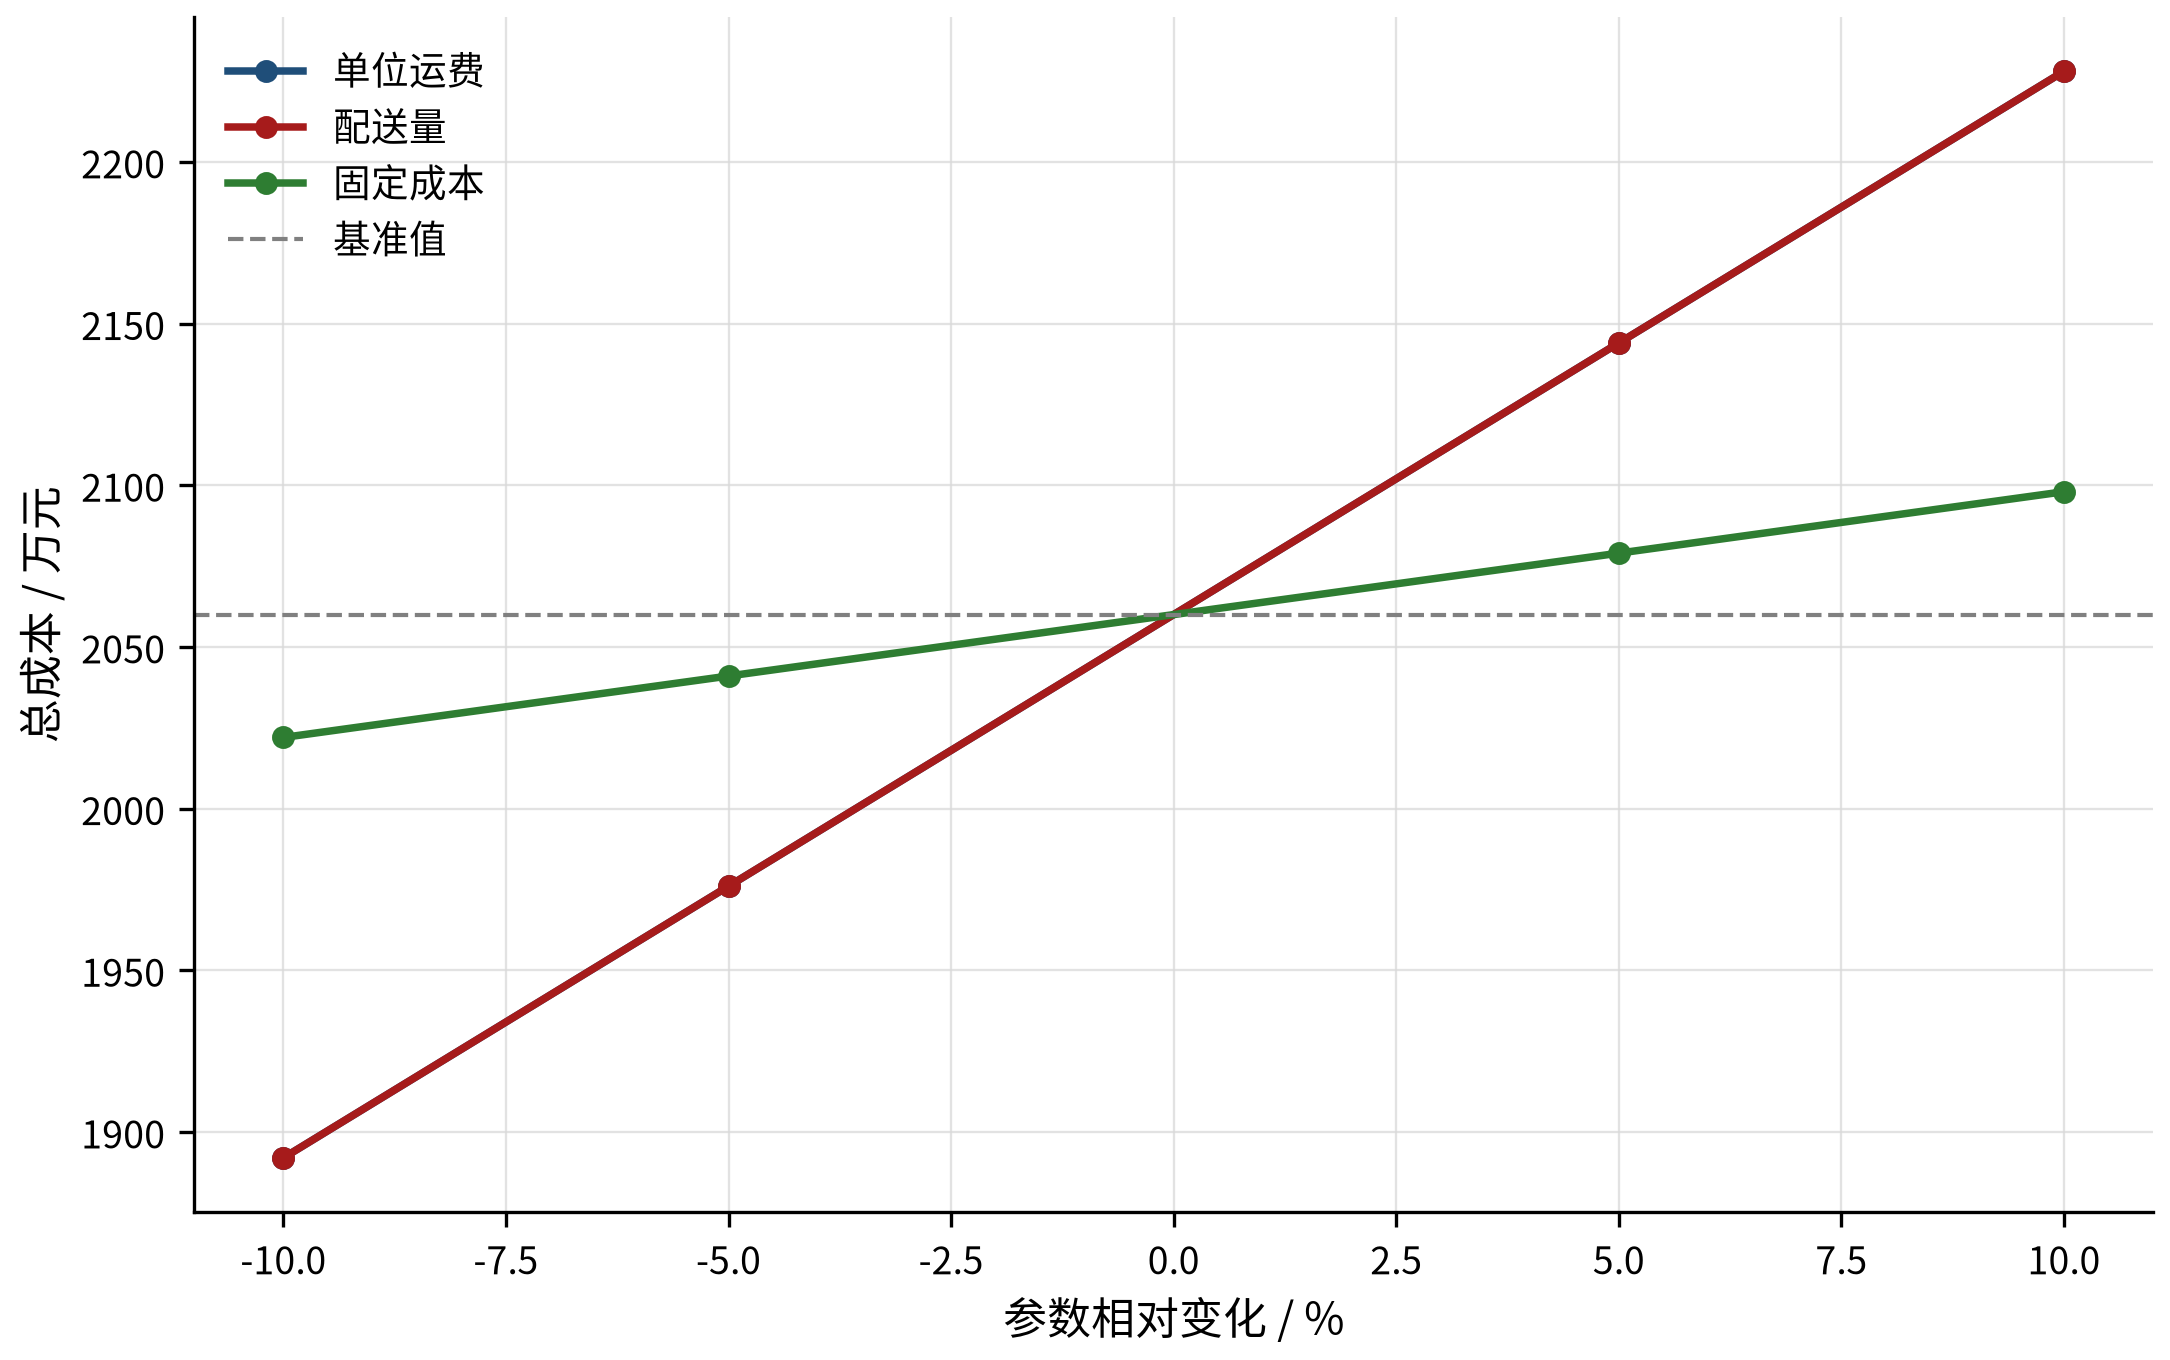
\includegraphics[width=0.8\textwidth]{fig2_sens.png}
  \caption{总成本对各参数扰动的响应曲线}
  \label{fig:sens}
\end{figure}

单位运费与配送量的弹性系数均为 0.8155，固定成本为 0.1845。二者之和恰为 1，这与成本函数的线性可加结构一致：可变成本占基准总成本的比例即为其弹性。前两个参数弹性相同，源于它们在模型中以乘积形式对称出现。在 $\pm 10\%$ 扰动下总成本波动区间为 1892.00--2228.00 万元，最大偏离基准 8.16\%，未出现放大效应，模型稳健。

\FloatBarrier

\section{模型评价与推广}

\subsection{模型的优点}

\begin{enumerate}
  \item 预测环节针对小样本特点选用 GM(1,1)，并完整执行了级比检验与残差检验，MAPE 仅 0.3592\%，精度可靠；
  \item 评价环节对正向化方式作了专门论证，用数据说明 $\max(x)-x$ 会使熵权失衡（0.9614 对 0.4904），避免了该方法常见的隐性错误；
  \item 第三问将复合问题拆解为最小生成树、最短路、线性规划三个标准模型，各自有成熟算法保证全局最优，避免了启发式方法的收敛不确定性；
  \item 全部结果附灵敏度分析，弹性系数之和为 1 的性质可作为计算正确性的交叉验证。
\end{enumerate}

\subsection{模型的缺点}

\begin{enumerate}
  \item GM(1,1) 仅刻画单调指数趋势，无法捕捉周期性波动；若未来产量出现拐点，预测将系统性偏高；
  \item 熵权法在方案数仅为 3 的情况下权重稳定性有限，样本增多时权重可能改变，实践中宜与 AHP 主观权重组合使用；
  \item 线性规划假设单位运费恒定，未考虑规模折扣与车辆整数约束，实际调度中应改用整数规划；
  \item 配送网络假设路段双向对称，未纳入单行道、限行时段与实时路况。
\end{enumerate}

\subsection{模型的推广}

本文的“预处理--预测--评价--优化--检验”框架不依赖具体行业背景，可直接迁移至冷链医药配送、应急物资储备点选址、快递分拨中心规划等场景。若数据量增大，问题一可替换为 ARIMA 或 BP 神经网络；若指标间存在强共线性，问题二可先做主成分分析降维；若需考虑车辆容量与时间窗，问题三可扩展为带容量约束的车辆路径问题（CVRP），用遗传算法或模拟退火求解。

\begin{thebibliography}{9}
\bibitem{ref1} 邓聚龙. 灰色系统基本方法[M]. 武汉: 华中科技大学出版社, 2005.
\bibitem{ref2} 司守奎, 孙兆亮. 数学建模算法与应用[M]. 3 版. 北京: 国防工业出版社, 2021.
\bibitem{ref3} Hwang C L, Yoon K. Multiple Attribute Decision Making: Methods and Applications[M]. Berlin: Springer, 1981.
\bibitem{ai-codex} OpenAI. Codex CLI, 0.146.0, OpenAI, 使用日期: 2026-08-01.
\end{thebibliography}

\begin{aideclaration}[AI 工具使用声明]

本文为工具箱示范材料。写作与程序组织过程中使用 OpenAI Codex 辅助生成和修改代码、整理文字；所有模型计算与数值结果均可由本项目代码重新生成，正式参赛时仍须按人工核对清单由队员复核后定稿。
\end{aideclaration}

\appendix
\section{支撑文件/材料清单}

\begin{table}[!htbp]
  \centering
  \small
  \caption{支撑材料清单}
  \label{tab:support}
  \begin{tabular}{lll}
    \toprule
    文件名 & 类型 & 说明 \\
    \midrule
    \texttt{compute.py} & Python 源码 & 全部计算，输出 \texttt{results.json} \\
    \texttt{results.json} & 数据 & 论文所有数值的唯一来源 \\
    \texttt{gen\_paper.py} & Python 源码 & 由 JSON 生成本文，杜绝手抄误差 \\
    \texttt{fig0\_workflow.png} & 图片 & 总体研究流程图 \\
    \texttt{fig1\_fit.png} & 图片 & 预测拟合与残差图 \\
    \texttt{fig2\_sens.png} & 图片 & 灵敏度分析图 \\
    \texttt{fig3\_net.png} & 图片 & 配送网络图 \\
    \bottomrule
  \end{tabular}
\end{table}

\section{程序代码}

全部计算由 \texttt{compute.py} 完成，共调用工具箱 \texttt{snippets/} 下的七个模块：

\begin{table}[!htbp]
  \centering
  \small
  \caption{程序调用的工具箱模块}
  \label{tab:modules}
  \begin{tabular}{ll}
    \toprule
    模块 & 本文中承担的工作 \\
    \midrule
    \texttt{preprocessing} & 缺测值插值填补、IQR 异常值检测 \\
    \texttt{grey\_prediction} & GM(1,1) 建模与外推 \\
    \texttt{model\_validation} & 残差统计、单因素灵敏度分析 \\
    \texttt{topsis\_entropy} & 熵权赋权与 TOPSIS 排序 \\
    \texttt{graph\_shortest\_path} & 最短路、最小生成树 \\
    \texttt{linear\_programming} & 运量分配线性规划 \\
    \texttt{plotting} & 拟合对比图、灵敏度曲线 \\
    \bottomrule
  \end{tabular}
\end{table}

运行方式（在仓库任意目录下执行均可，脚本自行定位仓库根）：

\begin{center}
\texttt{.venv/bin/python examples/示范论文/compute.py}
\end{center}

\end{document}
